\documentclass{article}

% packages
\usepackage[LGR]{fontenc}
\usepackage[english,greek]{babel}
\usepackage[left=4cm, right=4cm]{geometry}
\usepackage{amsfonts}
\usepackage{mathtools}
\usepackage{pifont}
\usepackage{amsmath}
\usepackage{listings}
\usepackage{lipsum}

% commands
\newcommand{\blank}[1]{\hspace*{#1}}
\newcommand{\mysp}{\blank{0.3cm}}
\newcommand{\lt}[1]{\latintext #1\greektext}
\newcommand{\gt}[1]{\greektext #1\latintext}
\newcommand{\blt}[1]{\lt{\textbf{#1}}}
\newcommand{\tb}[1]{\textbf{#1}}
\newcommand{\ti}[1]{\textit{#1}}
\newcommand{\lorem}{\lt{\lipsum[1]}}
\newcommand{\protege}{\lt{Prot\'eg\'e}}

% default parameters
\setlength{\parindent}{0pt}

% header
\title{\begin{flushright}
    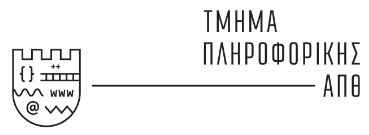
\includegraphics[scale=0.5]{images/authstamp.png}
    \quad
    \tb{Ανάπτυξη Οντολογίας Χημικού Εργοστασίου σε \protege}
\end{flushright}}

\author{
    Αποστολούδης Αντώνης\\
    3897\\
    \texttt{\lt{antoapos@csd.auth.gr}}
    \and
    Δροσσάς Ιωάννης\\
    3890\\
    \texttt{\lt{idrossas@csd.auth.gr}}
    \and
    Κύδρος Ασημάκης\\
    3881\\
    \texttt{\lt{asimakis@csd.auth.gr}}
}
\date{\today}

% body
\begin{document}
\maketitle

\section*{Περίληψη}
Χωρίσαμε το πρόβλημα σε 4 μεγάλες δομικές μονάδες: τα Χημικά (\lt{Chemical}), τα Φρεάτια (\lt{Drain}), τις Αποθήκες (\lt{Warehouse}) και τον σταθμό ελέγχου (\lt{ControlStation}). Κάθε μια από αυτές τις οντολογίες χαρακτηρίζεται με μία κλάση.\\

Βάσει των ιδιοτήτων που ονομάζονται στην εκφώνηση, διαχωρίσαμε περαιτέρω τα Χημικά σε τρεις υποκατηγορίες, τα Οξέα (\lt{Acid}), τις Βάσεις (\lt{Base}) και τα Έλαια (\lt{Oil}). Στενεύοντας τα όρια του \lt{pH}, εξειδικεύσαμε περαιτέρω τα οξέα και τις βάσεις σε Ισχυρά (\lt{StrongAcid, StrongBase}) και Ασθενή (\lt{WeakAcid, WeakBase}).

\newpage

\section*{Κλάσεις}
    \blt{Chemical:} Η κλάση αυτή αποτελεί το ανώτερο \lt{abstraction} για τα χημικά. Κάθε εξειδικευμένη ουσία είναι και χημικό. Επομένως, καλύπτει όλες τις δεδομένες ιδιότητες, δηλαδή έχει \lt{pH (Float single in range[0.0, 14.0])}, \lt{solubility (String)}, \lt{spectroscopy (String mulitple)}, \lt{colour (String required single)}, \lt{smell (String required single)}, \lt{specificGravity (Float required single in range[0.9, 1.1])}, \lt{radioactivity (Boolean required single)}. Επιπλέον προσθέσαμε και \lt{name (String required single)}, \lt{effects (String multiple)}, \lt{symbol (String single)}. Αυτά δρουν ως το μοναδικό \lt{id} του χημικού, τα πιθανά περίεργα \lt{extra} φαινόμενα που παρουσιάζει το χημικό, και ο χημικός του συμβολισμός αντιστοίχως.
    \begin{enumerate}
        \item \blt{Acid:} Η κλάση αυτή αναπαριστά όλα τα οξέα. Εξειδικεύει το εύρος του \lt{pH} σε (0.0, 5.999) και το \lt{solubility} σε \lt{soluble}.
        \begin{enumerate}
            \item \blt{StrongAcid:} Έτσι χαρακτηρίζονται τα ισχυρά οξέα. Το εύρος του \lt{pH} γίνεται ακόμα πιο αυστηρό, σε (0.0, 2.999) και αποκτά 2 \lt{effects}, το \lt{burn skin} και το \lt{corrosive}. 
            \item \blt{WeakAcid:} Με παρόμοιο τρόπο χαρακτηρίζονται και τα ασθενή οξέα, με εύρος \lt{pH} στο (3.0, 5.999).
        \end{enumerate}
        \item \blt{Base:} Η κλάση αυτή αναπαριστά τις Βάσεις. Σύμφωνα με τα δεδομένα, έχει εύρος \lt{pH} (8.0, 14.0) και είναι \lt{soluble}.
        \begin{enumerate}
            \item \blt{StrongBase:} Οι ισχυρές βάσεις έχουν επιπλέον εύρος \lt{pH} στο (11.0, 14.0) και είναι \lt{corrosive}.
            \item \blt{WeakAcid:} Παρομοίως, οι ασθενείς βάσεις μοντελοποιούνται με αυτή τη κλάση, που έχει εύρος \lt{pH} (8.0, 10.999).
        \end{enumerate}
        \item \blt{Oil:} Τέλος τα Έλαια μοντελοποιούνται με αυτή την κλάση, που φέρει εύρος \lt{pH} (6.0, 7.99) και είναι \lt{insoluble}. Δεν έχει περαιτέρω παιδιά.
    \end{enumerate}
    
    \blt{Warehouse:} Οι αποθήκες είναι απλές κλάσεις που αποσκοπούν στο να επισημάνουν την διατήρηση και τη ροή των χημικών μέσα στο εργοστάσιο. Έχουν μια απλή ιδιότητα, το \lt{warehouseName (String required single)}, που αποσκοπεί ως το όνομα-μοναδικό \lt{id} της αποθήκης.\\
    
    \blt{Drain:} Παρόμοια λογική ακολουθούν και τα φρεάτια, που φέρουν την αντίστοιχη ιδιότητα \lt{drainTitle (String required single)}.\\
    
    \blt{ControlStation:} Και τέλος ο σταθμός ελέγχου, παρόλο που είναι μοναδικός, χαρακτηρίζεται με μια κλάση ίδιας φιλοσοφίας, που έχει μονάδα ένα όνομα-id \lt{stationTitle (String required single)}. 

\newpage

\section*{Αντικείμενα}
Σύμφωνα με τις οδηγίες τις εκφώνησης, κάθε κλάση έχει τα εξείς αντικείμενα:\\

$\mysp\blt{StrongAcid} \rightarrow \blt{Hydrochloric Acid, Sulphuric Acid}$\\
$\mysp\blt{WeakAcid} \rightarrow \blt{Acetic Acid, Carbonic Acid}$\\
$\mysp\blt{StrongBase} \rightarrow \blt{Sodium Hydroxide}$\\
$\mysp\blt{WeakBase} \rightarrow \blt{Aluminum Hydroxide, Chromogen 23, Rubidium Hydroxide}$\\
$\mysp\blt{Oil} \rightarrow \blt{Petrol, Transformer Oil}$\\
$\mysp\blt{Warehouse} \rightarrow \blt{Warehouse 1, Warehouse 2, \dots, Warehouse 8}$\\
$\mysp\blt{Drain} \rightarrow \blt{Drain 1, Drain 2, \dots, Drain 13}$\\
$\mysp\blt{ControlStation} \rightarrow \blt{Station 1}$\\

Καταλήγουμε δηλαδή στο παρακάτω δέντρο:
\begin{center}
    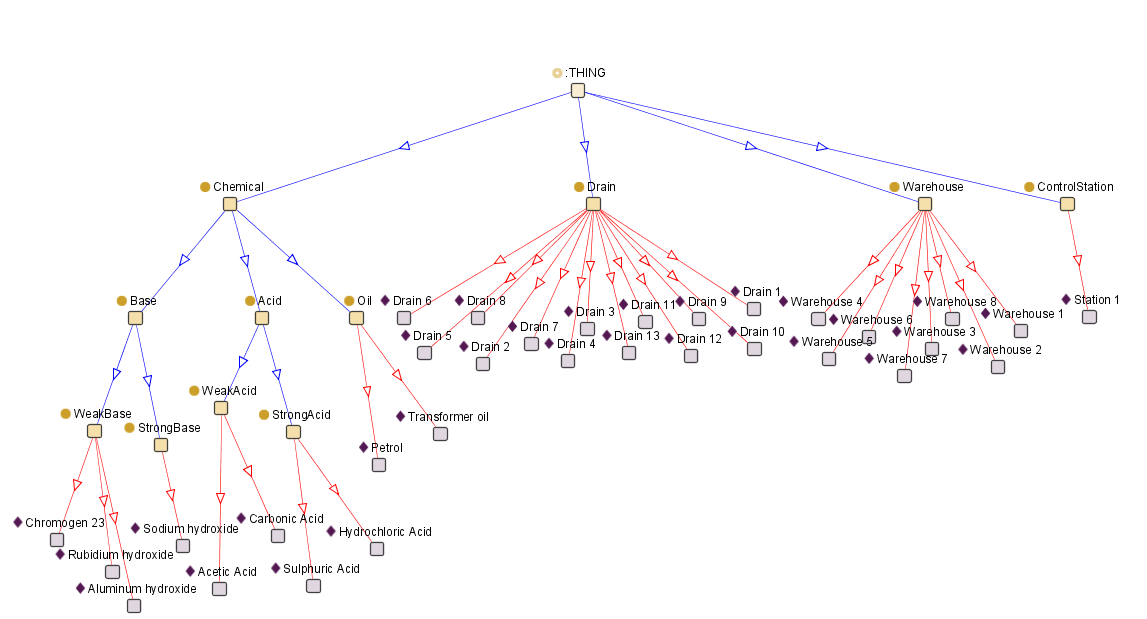
\includegraphics[scale=0.35]{images/class-instance tree.png}
\end{center}

\newpage

\section*{Σχέσεις}
Ακολουθούμενοι τον γράφο ροής των χημικών της εκφώνησης, ορίσαμε σχέσεις μεταξύ των κλάσεων. Αυτές είναι:

\begin{enumerate}
    \item \blt{LeaksTo}, με αντίστροφη την \blt{LeakedFrom}, που ορίζει την διαφυγή κάποιου χημικού από την αποθήκη \lt{i} στο φρεάτιο \lt{i}.
    \item \blt{DrainsTo}, με αντίστροφη την \blt{DrainedFrom}, που ορίζει την περαιτέρω διαφυγή του χημικού από το φρεάτιο \lt{i} στο φρεάτιο \lt{j}. Τα φρεάτια που φέρουν τέτοια σχέση είναι:
    \begin{enumerate}
        \item $\blt{Drain 1, Drain 2, Drain 3} \rightarrow \blt{Drain 9}$
        \item $\blt{Drain 4, Drain 5} \rightarrow \blt{Drain 10}$
        \item $\blt{Drain 6, Drain 7} \rightarrow \blt{Drain 11}$
        \item $\blt{Drain 8} \rightarrow \blt{Drain 13}$
        \item $\blt{Drain 9, Drain 10} \rightarrow \blt{Drain 12}$
        \item $\blt{Drain 11} \rightarrow \blt{Drain 13}$
    \end{enumerate}
    \item \blt{DetectedFrom}, με αντίστροφη την \blt{Detects}, που ορίζει τον εντοπισμό της διαφυγής του χημικού από το φρεάτιο \lt{i} στον σταθμό ελέγχου. Τα φρεάτια που φέρουν τέτοια σχέση είναι $\blt{Drain 12, Drain 13} \rightarrow \blt{Station 1}$
\end{enumerate}

\end{document}
